\pagestyle{headings}
\chapter{Point Estimation} \label{chp 6}
\thispagestyle{fancy}

\subsection*{Introduction: The German Tank Problem}\index{German Tank Problem}

During the course of a war, three enemy tanks of a particular type are captured. Each tank has a serial number printed inside it. The first tank of this type to have been produced has serial number one, the second has serial number two, and so on. 
\par
The serial numbers found in the three tanks are 121, 53, and 246. What is your best guess at the total number of tanks of this type that have been produced?
\par
The task of making a single guess at an unknown quantity, using information in a sample, is known as point estimation. Note that the point estimation problem above is very open-ended. What exactly does it mean to answer correctly?
%\par
%\begin{itemize}
%\item The largest value, $246$ is one guess, though it's going to be an underestimate unless we happen to capture the most recently produced tank.
%\item Take the average, $\frac{1}{3}(121+53+246) = 140$. If a total of $n$ tanks have been produced, then the average serial number will be $\frac{n}{2}$, so we can double our average to obtain an estimate of $280$.
%\item Consider laying out the sample on a number line and measuring the gaps between values. There's an initial gap of $53$, then $121-53 = 68$, and then $246-121 = 125$. The average gap is $\frac{1}{3}(53+68+121) = 82$. If we add this average gap to the highest value in the sample, we obtain $328$.
%\end{itemize}
\par

\section{Statistics \& Parameters}

\begin{definition}\index{Statistic}\index{Parameter}
A parameter is a numerical property of a population being studied, and a statistic is a numerical property of a sample taken from this population.
\end{definition}
\par
The key idea is to always distinguish between values obtained from complete information, with no uncertainty, and those obtained from incomplete information via some sampling process.
\begin{examp}\label{ClassAge}
If we wish to estimate the average age of all students in a classroom, the population in question is the set of all students in the room. Their average age is the parameter we want to estimate. If we ask a randomly selected group of five students their ages and average those, the value obtained is a statistic.
\end{examp}
\begin{examp}
In the German tank problem given in the introduction to this chapter, the population being studied is the set of all tanks of a particular type. Each serial number is represented once, so the distribution of serial numbers in the population is $Uniform(m)$, where $m$, the largest serial number, is the parameter we would like to estimate. Any value which can be derived from the given sample of three serial numbers we were given will be a statistic.
\end{examp}
\par
The central theme of inferential statistics is how to use statistics which we know to estimate parameters which we don't, and how to quantify the inherent error in our estimation methods. In many fields, sample information is the only information we have access to, and decisions must be made based on it. This makes inferential statistics a necessary tool over an extremely wide range of applications.

%\begin{examp}
%In order to try to determine the most common number of hours of sleep per night blahblah
%\end{examp}

\section{Sampling Distributions \& Estimators}

The value of a statistic is determined by the sample it was derived from, and hence \emph{a statistic is a function whose input is a sample, and whose output is a number}.
\par
If we fix a sample size, $n$, define a sample space $\Omega$ as the set of possible samples of that size, and assign probabilities to each possible sample, then any statistic that can be computed from a sample of size $n$ is a random variable defined on $\Omega$ (recall Definition \ref{RandomVariableDef}). This is the central idea of frequentist statistics: a parameter is simply a value which may or may not be known, but a \emph{statistic is a random variable} and like any random variable, \emph{it has a distribution}.

\begin{defn}\index{Sampling Distribution}
The sampling distribution of a statistic, over samples of size $n$, is the distribution of possible values of that statistic.
\end{defn}

\begin{examp}\label{MeanAgeEx} Consider a population of three individuals, Alice, Bob, and Charles. Alice is 12 years old, Bob is 16 years old, and Charles is 22 years old. Let $\overline{X}$ denote the mean age in a sample of two individuals drawn from this population ($\overline{X}$ is standard notation for a sample mean in statistical practice). Find the sampling distribution of $\overline{X}$ over all samples of size two taken with replacement.
\par
\noindent If we let $X_1$ and $X_2$ denote the ages of the first and second individuals selected in our sample, then $\overline{X} = \frac{1}{2}(X_1 + X_2)$. There are $3\cdot3 = 9$ possible samples, which we enumerate below and for each, calculate the value of $\overline{X}$.

\begin{center}
\begin{tabular}{c|c|c|c}
Sample & $X_1$ & $X_2$ & $\overline{X}$ \\
\hline
A,A & $12$ & $12$ & $12$ \\
A,B & $12$ & $16$ & $14$ \\
A,C & $12$ & $22$ & $17$ \\
B,A & $16$ & $12$ & $14$ \\
B,B & $16$ & $16$ & $16$ \\
B,C & $16$ & $22$ & $19$ \\
C,A & $22$ & $12$ & $17$ \\
C,B & $22$ & $16$ & $19$ \\
C,C & $22$ & $22$ & $22$ \\
\end{tabular}
\end{center}

\par
\noindent If we assume every sample is equally likely, then each sample above occurs with probability $\frac{1}{9}$, so we obtain the sampling distribution below.

\vspace{-1em}
\begin{center}
    \begin{minipage}{.45\textwidth}
        \centering
      \renewcommand*{\arraystretch}{1.35}
\begin{tabular}{c|c}
$\overline{X}$ & $P(\overline{X} = \overline{x})$ \\
\hline
12 & $\frac{1}{9}$ \\
14 & $\frac{2}{9}$ \\
16 & $\frac{1}{9}$ \\
17 & $\frac{2}{9}$ \\
19 & $\frac{2}{9}$ \\
22 & $\frac{1}{9}$
\end{tabular}
\renewcommand*{\arraystretch}{1}
\vspace{0.25em}
    \end{minipage}%
    \begin{minipage}{0.5\textwidth}
        \centering
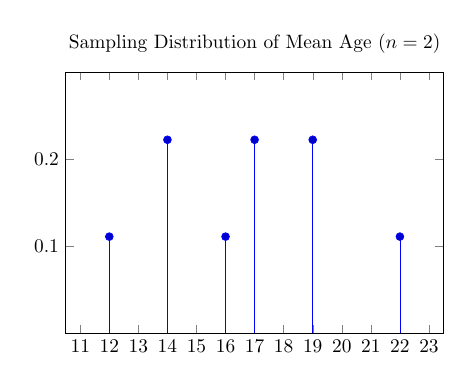
\begin{tikzpicture}[scale = 0.7]
\begin{axis} [title = {Sampling Distribution of Mean Age ($n=2$)}, unit vector ratio=1 30 1, ymin = 0, ymax = 0.3, xmin = 10.5, xmax = 23.5,
		ytick = {0.1,0.2}, xtick = {11,12,13,14,15,16,17,18,19,20,21,22,23}]
\addplot+[ycomb] plot coordinates {(12,0.1111) (14,0.2222) (16,0.1111) (17,0.2222) (19,0.2222) (22,0.1111)}; 
\end{axis}
\end{tikzpicture}
\end{minipage}
\end{center}
\end{examp}

\subsection*{Random Sampling}\index{Random Sample}

To compute the sampling distribution above, we assumed every sample was equally likely. The sampling distribution depends on the sampling process, so we must be explicit about what constitutes a sample and how samples are selected.

\begin{defn}\index{Simple Random Sample} (SRS Informally) If an ordered sequence of individuals is selected in a manner where every member of the population is equally likely to be chosen for each position in the sequence, we obtain a simple random sample (SRS) taken with replacement.
\end{defn}
\rmk SRSs can also be taken without replacement. Sampling with replacement and without replacement are both common in practice, and the most important results we'll derive apply when sampling without replacement as well.
\par
In Example \ref{MeanAgeEx} above, consider the distribution of age in the population. There is a single 12 year old, a single 16 year old, and a single 22 year old, so if $X$ denotes the age of an individual selected uniformly at random from the population, then the distribution of $X$ is given below.

\begin{center}
    \begin{minipage}{.45\textwidth}
       \centering
      \renewcommand*{\arraystretch}{1.35}
\eqnspar{f_X(x) = \left\{
\begin{array}{cl}
      \frac{1}{3} & \text{ if \ } x = 12 \\
			\frac{1}{3} & \text{ if \ } x = 16 \\
			\frac{1}{3} & \text{ if \ } x = 22 \\
      0 & \text{ otherwise }  \end{array}
\right.}
\renewcommand*{\arraystretch}{1}
\vspace{1em}
    \end{minipage}%
    \begin{minipage}{0.5\textwidth}
        \centering
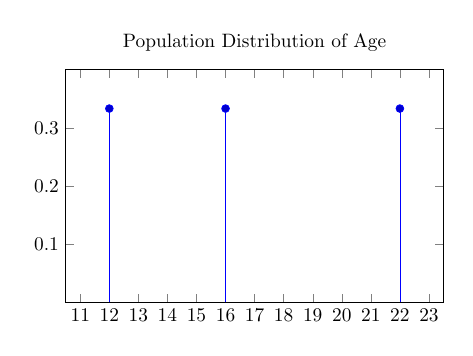
\begin{tikzpicture}[scale = 0.7]
\begin{axis} [title = {Population Distribution of Age}, unit vector ratio=1 20 1, ymin = 0, ymax = 0.4, xmin = 10.5, xmax = 23.5,
		ytick = {0.1,0.2,0.3}, xtick = {11,12,13,14,15,16,17,18,19,20,21,22,23}]
\addplot+[ycomb] plot coordinates {(12,0.33333) (16,0.33333) (22,0.33333)}; 
\end{axis}
\end{tikzpicture}
\end{minipage}
\end{center}

\par
In a SRS (with replacement) of two individuals taken from this population, the first individual chosen must be equally likely to be Alice, Bob, or Charles, the second individual chosen must also be equally likely to be Alice, Bob, or Charles, and so on. If $X_i$ represents the age of the $i^{th}$ individual in our sample, then $X_i$ must have the distribution given above, and moreover, knowledge of the value of $X_i$ should not influence our beliefs about any $X_j$ for $i \neq j$.
\par
\begin{defn}\label{FormalSRSDef}\index{Simple Random Sample} (SRS Formally) Given a distribution $X$, a simple random sample taken with replacement from $X$ is a sequence $X_1, X_2, ... \,, X_n$ of independent, identically distributed random variables, each of which has the same distribution as $X$.
\end{defn}

\begin{examp} Consider a population of four individuals, one has shoe size 7, one has shoe size 10, and the other two have shoe size 11. If a SRS of two individuals is taken with replacement from this population, what is the probability the second individual chosen has shoe size 11? If the first individual chosen has shoe size 10, what is the probability the second individual chosen has shoe size 11?
\par
\noindent Let $X$ denote the distribution of shoe sizes in the population, so $P(X = 7) = \frac{1}{4}$, $P(X = 10) = \frac{1}{4}$, and $P(X = 11) = \frac{1}{2}$.
\par
\noindent Our sample $X_1, X_2$ is a SRS taken with replacement, so the probability any $X_i$ is a 11 should be $\frac{1}{2}$, regardless of the values of any other $X_j$. Thus, $P(X_2 = 11) = P(X = 11) = \textstyle\frac{1}{2}$ and $P(X_2 = 11 \given X_1 = 10) = P(X_2 = 11) = \textstyle\frac{1}{2}$.
\end{examp}

\subsection*{Estimators}

When a statistic is being used to estimate a parameter, we call it an estimator\index{Estimator} for that parameter. Parameters are typically denoted with greek letters, such as $\theta$, and the notation $\widehat{\theta}$ is often used to denote a statistic estimating $\theta$.

\begin{examp}Suppose that in the context of Example \ref{MeanAgeEx}, the mean age in a SRS of size two is used to estimate the mean age in the population. The SRS selected consists of Alice and Charles. What are $\mu$ and $\widehat{\mu}$?
\par
\noindent The greek letter $\mu$ is typically used to denote a population mean, so in this scenario, we have the parameter $\mu = \frac{50}{3} \simeq 16.67$ and the estimator $\widehat{\mu} = \frac{1}{2}(X_1+X_2)$ which with our sample, gives the estimate $\widehat{\mu} = \frac{1}{2}(12+22) = 17$.
\end{examp}
\par
In this case, the value of our estimator ended up very close to $\mu$, which is exactly what we're hoping for. In practice though, we don't know the value of the parameter being estimated, or we wouldn't have been estimating it in the first place! Without this knowledge, how can we begin to evaluate the usefulness of an estimator?
\par
Notice that the sampling distribution of the sample mean $\overline{X}$ that we constructed in Example \ref{MeanAgeEx} has a very nice property. If we compute its expected value 
\eqnspar{E(\overline{X}) = 12\cdot \textstyle\frac{1}{9} +14\cdot \frac{2}{9} + 16\cdot \frac{1}{9} + 17\cdot \frac{2}{9} + 19\cdot \frac{2}{9} + 22\cdot \frac{1}{9} = \frac{150}{9} = \frac{50}{3}}
\par
\noindent the result is precisely equal to the population mean $\mu$. Thus, if we use the estimator $\widehat\mu = \overline{X} = \frac{1}{n}(X_1+X_2)$ to estimate the population mean, then the average value of our estimator is equal to the parameter $\mu$ being estimated. We say that $\widehat\mu = \overline{X}$ is an unbiased estimator of $\mu$.

\begin{defn}\label{Unbiased Estimator}\index{Unbiased Estimator}\index{Estimator!bias of} The \index{Estimator!bias of}bias of an estimator is the difference between its expected value and the actual value of the parameter being estimated.
$$\boxed{Bias(\widehat{\theta}) = E(\widehat{\theta}) - \theta}$$ 
\end{defn}
\par
If $Bias(\widehat{\theta}) > 0$, the mean value of $\widehat{\theta}$ is an overestimate of $\theta$, if $Bias(\widehat{\theta}) < 0$, the mean value of $\widehat{\theta}$ is an underestimate of $\theta$, and if $Bias(\widehat{\theta}) = 0$ then $E(\widehat{\theta}) = \theta$ and $\widehat{\theta}$ is an unbiased estimator of $\theta$.
\par
The concept of bias is fairly intuitive. Suppose you estimate the average age of all students in a classroom by finding the oldest student in the class and reporting their age. This estimator will have positive bias. Similarly, if you estimate the average age of all students in a classroom by finding the youngest student in the class and reporting their age, that estimator will have negative bias.

\begin{thm} In any population, the mean of a SRS taken with replacement is an unbiased estimator of the population mean $\mu$.
\end{thm}
\begin{pf} Let $\widehat{\mu} = \overline{X} = \frac{1}{n}(X_1 + X_2 + ... + X_n)$, where $X_i$ is the $i^{th}$ value in our sample.
\par
\noindent If our sample is a SRS taken with replacement, the distribution of each $X_i$ is the same as the population distribution. Therefore, $E(X_i) = E(X) = \mu$, the population mean, and by linearity of expectation,
\eqns{E(\widehat{\mu}) &= E(\textstyle\frac{1}{n}(X_1 + X_2 + ... + X_n)) \\
&= \textstyle\frac{1}{n}E(X_1 + X_2 + ... + X_n) \\
&= \textstyle\frac{1}{n}(E(X_1) + E(X_2) + ... + E(X_n)) \\ 
&= \textstyle\frac{1}{n}(\mu + \mu + ... + \mu) \\
& = \textstyle\frac{1}{n}(n \mu)\\
& = \mu.}
\end{pf}

\begin{examp}\label{MiniGermanTank}Consider a miniature version of the German Tank Problem given in the introduction to this chapter, where the population consists of only four tanks, with serial numbers 1 through 4. Let $\theta$ denote the population maximum, so $\theta = 4$. 
\par
\noindent If we estimate $\theta$ by taking the maximum serial number in a sample of size two, show we'll obtain a biased estimate. If we estimate $\theta$ by doubling the average serial number in a sample of size two then subtracting one, show we'll obtain an unbiased estimate.
\par
\noindent Define $\widehat{\theta}_1 = max(X_1,X_2)$ and \,$\widehat{\theta}_2 = 2 \cdot \frac{1}{2}(X_1 + X_2) - 1$. There are sixteen possible samples taken with replacement, so we have the samples and corresponding values of the two estimators given below.
\begin{center}
\begin{minipage}{0.5\textwidth}
\centering
\begin{tabular}{c|c|c|c}
$X_1$ & $X_2$ & $\,\widehat{\theta}_1\,$ & $\,\widehat{\theta}_2\,$ \\
\hline
$1$ & $1$ & $1$ & $1$ \\
$1$ & $2$ & $2$ & $2$ \\
$1$ & $3$ & $3$ & $3$ \\
$1$ & $4$ & $4$ & $4$ \\
$2$ & $1$ & $2$ & $2$ \\
$2$ & $2$ & $2$ & $3$ \\
$2$ & $3$ & $3$ & $4$ \\
$2$ & $4$ & $4$ & $5$ \\
$3$ & $1$ & $3$ & $3$ \\
$3$ & $2$ & $3$ & $4$ \\
$3$ & $3$ & $3$ & $5$ \\
$3$ & $4$ & $4$ & $6$ \\
$4$ & $1$ & $4$ & $4$ \\
$4$ & $2$ & $4$ & $5$ \\
$4$ & $3$ & $4$ & $6$ \\
$4$ & $4$ & $4$ & $7$ \\
\end{tabular}
\end{minipage}\begin{minipage}{0.5\textwidth}
\centering
\renewcommand*{\arraystretch}{1.23}
\begin{tabular}{c|c}
$x$ & $P(\widehat{\theta}_1 = x)$ \\
\hline
$1$ & $\frac{1}{16}$ \\
$2$ & $\frac{3}{16}$ \\
$3$ & $\frac{5}{16}$ \\
$4$ & $\frac{7}{16}$ \\
\end{tabular}
\ \\
\vspace{1em}
\ \\
\begin{tabular}{c|c}
$x$ & $P(\widehat{\theta}_2 = x)$ \\
\hline
$1$ & $\frac{1}{16}$ \\
$2$ & $\frac{2}{16}$ \\
$3$ & $\frac{3}{16}$ \\
$4$ & $\frac{4}{16}$ \\
$5$ & $\frac{3}{16}$ \\
$6$ & $\frac{2}{16}$ \\
$7$ & $\frac{1}{16}$ \\
\end{tabular}
 \renewcommand*{\arraystretch}{1}
\end{minipage}
\end{center}

\vspace{-1em}
\begin{center}
    \begin{minipage}{0.5\textwidth}
        \centering
     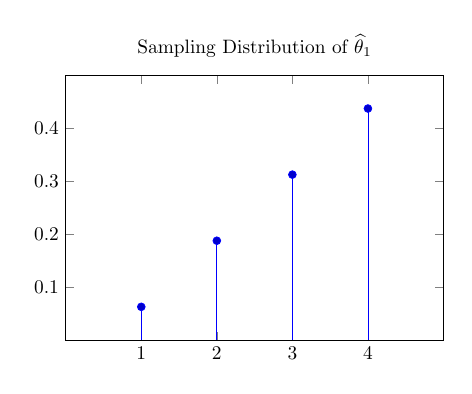
\begin{tikzpicture}[scale = 0.7]
\begin{axis} [title = {Sampling Distribution of $\widehat{\theta}_1$}, unit vector ratio=1 7 1, ymin = 0, ymax = 0.5, xmin = 0, xmax = 5,
		ytick = {0.1,0.2, 0.3,0.4}, xtick = {1,2,3,4}]
\addplot+[ycomb] plot coordinates {(1,0.0625) (2,0.1875) (3,0.3125) (4,0.4375)}; 
\end{axis}
\end{tikzpicture} \ \ 
    \end{minipage}%
    \begin{minipage}{0.5\textwidth}
        \centering
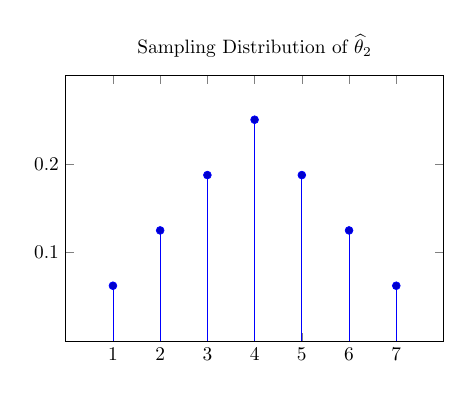
\begin{tikzpicture}[scale = 0.7]
\begin{axis} [title = {Sampling Distribution of $\widehat{\theta}_2$}, unit vector ratio=1 18.75 1, ymin = 0, ymax = 0.3, xmin = 0, xmax = 8,
		ytick = {0.1,0.2}, xtick = {1,2,3,4,5,6,7}]
\addplot+[ycomb] plot coordinates {(1,0.0625) (2,0.125) (3,0.1875) (4,0.25) (5,0.1875) (6,0.125) (7,0.0625)}; 
\end{axis}
\end{tikzpicture} \ \ 
\end{minipage}
\end{center}

\par
\noindent Now we can compute the expected values and evaluate the bias of each estimator.
\eqns{E(\widehat{\theta}_1) &= 1 \cdot \textstyle\frac{1}{16} + 2 \cdot \frac{3}{16} + 3 \cdot \frac{5}{16} + 4 \cdot \frac{7}{16} = \frac{50}{16} = \frac{25}{8} \\
E(\widehat{\theta}_2) &= 1 \cdot \textstyle\frac{1}{16} + 2 \cdot \frac{2}{16} + 3 \cdot \frac{3}{16} + 4 \cdot \frac{4}{16} + 5 \cdot \textstyle\frac{3}{16} + 6 \cdot \frac{2}{16} + 7 \cdot \frac{1}{16}= \frac{64}{16} = 4}
\par
\noindent Thus, $\text{Bias}(\widehat{\theta}_1) = \frac{25}{8} - 4 = -\frac{7}{8} = -0.875$ and $\text{Bias}(\widehat{\theta}_2) = 4 - 4 = 0$.

\end{examp}
\par
\rmk If the population we're studying is small, we can explicitly compute the sampling distribution by writing down every possible sample, as above. Of course, this is rarely feasible in practice. 

In general, the sampling distribution can be approximated by repeatedly taking random samples using a computer and recording the values of the relevant statistic. The distribution obtained will be a better and better approximation of the true sampling distribution as the number of samples grows larger and larger.

\section{Evaluating Estimators}

What determines whether an estimator produces useful estimates of a parameter, and what makes one estimator better than another? Clearly, good estimators should take values close to the parameter being estimated, so the smaller that the typical difference between the two is, the better.

%KEY POINT: An estimator is a way of computing a number from a sample, it's a RANDOM VARIABLE, which is a FUNCTION from samples to R. Evaluting the estimtor is determining whether thats a GOOD FUNCTION!

\begin{defn}\index{Mean-Squared Error}\index{Estimator!mean-squared error of} The mean-squared error of an estimator is the expected value of the squared difference between the estimator and the parameter it estimates.
\eqnsgap{\boxed{\text{MSE}(\widehat{\theta}) = E[(\widehat{\theta} - \theta)^2]}}
\end{defn}
\par
\noindent
\begin{examp}Find the MSE of the two estimators $\widehat{\theta}_1$ and $\widehat{\theta}_2$ in Example \ref{MiniGermanTank}.
\par
\noindent In both cases, the parameter being estimated is $\theta = 4$, and from the sampling distributions of $\widehat{\theta}_1$ and $\widehat{\theta}_2$, we can compute 
\eqnsgap{MSE(\widehat{\theta}_1) &= E[(\widehat{\theta}_1 - \theta)^2] \\ &= (1-4)^2 \cdot \textstyle\frac{1}{16} + (2-4)^2 \cdot \textstyle\frac{3}{16} + (3-4)^2 \cdot \textstyle\frac{5}{16} + (4-4)^2 \cdot \textstyle\frac{7}{16} \\ &=9 \cdot \textstyle\frac{1}{16} + 4 \cdot \textstyle\frac{3}{16} + 1 \cdot \textstyle\frac{5}{16} + 0 \cdot \textstyle\frac{7}{16} = \frac{26}{16} \\
MSE(\widehat{\theta}_2) &= E[(\widehat{\theta}_2 - \theta)^2] \\ &= (1-4)^2 \cdot \textstyle\frac{1}{16} + (2-4)^2 \cdot \textstyle\frac{2}{16} + (3-4)^2 \cdot \textstyle\frac{3}{16} + \ ... \ + (7-4)^2 \cdot \textstyle\frac{1}{16} \\ &=9 \cdot \textstyle\frac{1}{16} + 4 \cdot \textstyle\frac{2}{16} + 1 \cdot \textstyle\frac{3}{16} + 0 \cdot \textstyle\frac{4}{16} + 1 \cdot \textstyle\frac{3}{16} + 4 \cdot \textstyle\frac{2}{16} + 9 \cdot \textstyle\frac{1}{16} = \frac{40}{16}}
\end{examp}
\par

\begin{thm}\label{BiasVarianceDecomp}\index{Bias-Variance Decomposition}$\index{Estimator!variance of}\text{MSE}(\widehat{\theta}) = \text{Bias}^2(\widehat{\theta}) + \Var(\widehat{\theta})$, where $\Var(\widehat{\theta}) = E[(\widehat{\theta} - E(\widehat{\theta}))^2]$ 
\end{thm}
\begin{pf} The result follows from a calculation using linearity of expectation.
\eqns{\text{MSE}(\widehat{\theta}) &= E[(\widehat{\theta} - \theta)^2] \\
&= E[(\widehat{\theta} - E[\widehat{\theta}] + E[\widehat{\theta}] -  \theta)^2] \\
&= E[(\widehat{\theta} - E[\widehat{\theta}])^2 + 2(\widehat{\theta} - E[\widehat{\theta}]) (E[\widehat{\theta}] - \theta) + (E[\widehat{\theta}] - \theta)^2] \\
&= E[(\widehat{\theta} - E[\widehat{\theta}])^2] + E[2(\widehat{\theta} - E[\widehat{\theta}]) (E[\widehat{\theta}] - \theta)] + E[(E[\widehat{\theta}] - \theta)^2] \\
&= E[(\widehat{\theta} - E[\widehat{\theta}])^2] + E[2(\widehat{\theta} - E[\widehat{\theta}]) (E[\widehat{\theta}] - \theta)] + (E[\widehat{\theta}] - \theta)^2 \\
&= \Var(\widehat{\theta}) + E[2(\widehat{\theta} - E[\widehat{\theta}]) \text{Bias}(\widehat{\theta}) ] + \text{Bias}^2(\widehat{\theta})  \\
&=\Var(\widehat{\theta}) + 2\text{Bias}(\widehat{\theta}) \cdot E[\widehat{\theta} - E(\widehat{\theta})]+ \text{Bias}^2(\widehat{\theta})  \\
&=\Var(\widehat{\theta}) + 2\text{Bias}(\widehat{\theta})\cdot (E[\widehat{\theta}] - E[E(\widehat{\theta})]) + \text{Bias}^2(\widehat{\theta})  \\
&=\Var(\widehat{\theta}) + 2\text{Bias}(\widehat{\theta})\cdot (E[\widehat{\theta}] - E[\widehat{\theta}]) + \text{Bias}^2(\widehat{\theta})  \\
&=\text{Bias}^2(\widehat{\theta}) + \Var(\widehat{\theta})  \\}
\end{pf}
\par
The bias of an estimator measures the distance between the mean of the sampling distribution and the parameter being estimated, while the variance measures the dispersion in the sampling distribution.

\begin{center}
    \begin{minipage}{0.5\textwidth}
        \centering
     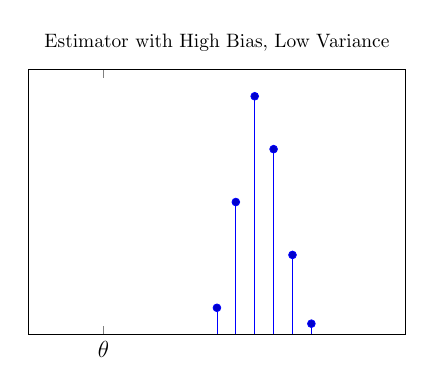
\begin{tikzpicture}[scale = 0.7]
\begin{axis} [title = {Estimator with High Bias, Low Variance}, unit vector ratio=1 7 1, ymin = 0, ymax = 0.5, xmin = 0, xmax = 5,
		 ytick = \empty, xtick = {1}, xticklabel = {\large$\theta$}]
\addplot+[ycomb] plot coordinates {(2.5,0.05) (2.75,0.25) (3,0.45) (3.25,0.35) (3.5,0.15) (3.75,0.02)}; 
\node at (axis cs:2,-0.1){\large$\theta$};
\end{axis}
\end{tikzpicture} \ \ 
    \end{minipage}%
    \begin{minipage}{0.5\textwidth}
        \centering
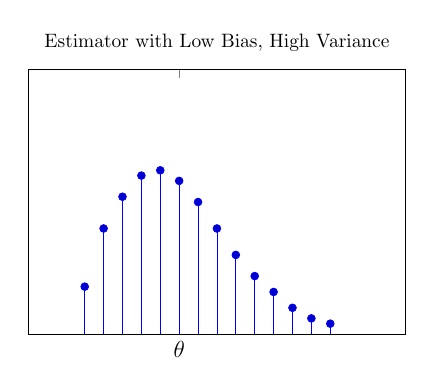
\begin{tikzpicture}[scale = 0.7]
\begin{axis} [title = {Estimator with Low Bias, High Variance}, unit vector ratio=1 7 1, ymin = 0, ymax = 0.5, xmin = 0, xmax = 5,
		ytick = \empty, xtick = {2}, xticklabel = {\large$\theta$}]
\addplot+[ycomb] plot coordinates {(0.75,0.09)(1,0.2) (1.25,0.26) (1.5,0.3) (1.75,0.31) (2,0.29) (2.25, 0.25) (2.5,0.2) (2.75,0.15) (3,0.11) (3.25,0.08) (3.5,0.05) (3.75,0.03) (4,0.02)}; 
\end{axis}
\end{tikzpicture} \ \ 
\end{minipage}
\end{center}

\par
Consider as an analogy an archery contest in which five shots are taken by each competitor. Estimators with high bias and low variance are akin to archers whose five arrows fall very close together, but all land quite far from the target. Estimators with low bias and high variance are akin to archers whose arrows are centred around the middle of the target, but with each individual arrow potentially landing quite far from it.
\par
The best estimators are those whose values centre around the parameter being estimated and also vary as little as possible. That is, those with low bias and low variance. Theorem \ref{BiasVarianceDecomp} assures us that an estimator with both these properties will also have a small mean-squared error.

\begin{examp} Consider the Mini German Tank Problem in Example \ref{MiniGermanTank}. Find the mean-squared error, bias, and variance of the estimators $\widehat{\theta}_1$ and $\widehat{\theta}_2$ whose sampling distributions we calculated.
\par
\noindent We already have $MSE(\widehat{\theta}_1) =\frac{26}{26}$ and $\text{Bias}(\widehat{\theta}_1) =-\frac{7}{8}$ from our earlier calculations, so by Theorem \ref{BiasVarianceDecomp}, we have
\eqns{\text{MSE}(\widehat{\theta}_1) &= Bias^2(\widehat{\theta}_1) + \Var(\widehat{\theta}_1)\\
\textstyle\frac{26}{16} &= (-\textstyle\frac{7}{8})^2 + \Var(\widehat{\theta}_1) \\
Var(\widehat{\theta}_1) &= \textstyle\frac{55}{64}.}
\par
\noindent Since $\widehat{\theta}_2$ is unbiased, $\text{MSE}(\widehat{\theta}_2) = \Var(\widehat{\theta}_2)$ by Theorem \ref{BiasVarianceDecomp}, so $\Var(\widehat{\theta}_2) = \frac{40}{16}$. Note that $\widehat{\theta}_1$ is the estimator with the lower $\text{MSE}$ despite the fact that it's biased.
\end{examp}

\section{Maximum Likelihood Estimation}

One strategy for estimating a parameter from sample data is to determine the value that makes the observed sample as likely as possible to occur. If I told you that in a sample of $50$ flips of a biased coin, $40$ heads and $10$ tails occurred, then $\frac{40}{50} = 0.8$ clearly seems like the best guess you could make for the probability of heads on a single flip of that coin. This value is called a maximum likelihood estimate\index{Maximum Likelihood Estimator}.

\begin{defn}\index{Likelihood Function}Suppose we have a SRS taken with replacement $x_1, x_2, ... \,,x_n$ from a population distribution $X$ with an unknown parameter $\theta$. The likelihood function for this sample is denoted $\mathcal{L}(x_1,x_2,...\,,x_n \given \theta)$ and defined by
\eqnsgap{\boxed{\mathcal{L}(x_1,x_2,...\,,x_n \given \theta) = f_X(x_1)f_X(x_2)...f_X(x_n) = \prod_{i=1}^{n}f_X(x_i)}}
\end{defn}
\par
Since our sample is a SRS, $f_X(x_1)f_X(x_2)...f_X(x_n)$ is the probability (or probability density) of observing the sample values $X_1 = x_1, X_2  = x_2, ...\,, X_n = x_n$. The maximum likelihood estimate is the value of $\theta$ that maximizes $\mathcal{L}(x_1,x_2,...\,,x_n \given \theta)$.
\par
We can use familiar techniques from differential calculus to find the maximum. One useful trick to recall is that because $\ln(x)$ is an increasing function, the value of $\theta$ that maximizes $\mathcal{L}(x_1,x_2,...\,,x_n \given \theta)$ will also maximize $\ln(\mathcal{L}(x_1,x_2,...\,,x_n \given \theta))$. This will greatly simplify calculations since the logarithm of a product can be written as a sum of logarithms, and derivatives of sums are much easier to deal with. To take advantage of this, let's denote the log-likelihood with $\ell(x_1,x_2,...\,,x_n \given \theta)$\index{Log-Likelihood Function}.
\eqns{\boxed{\ell(x_1,x_2,...\,,x_n \given \theta) = \ln\left(f_X(x_1)f_X(x_2)...f_X(x_n)\right) = \sum_{i=1}^{n}\ln\left(f_X(x_i)\right)}}

\begin{examp}
Let $X \sim Exponential(\lambda)$, and suppose we observe a SRS of three values from this distribution with $X_1 = 1, X_2 = 3, X_3 = 4$. Find the maximum likelihood estimate of $\lambda$.
\par
\noindent Note that $\lambda \in (0,\infty)$ for an exponential distribution. To begin with, we'll write out the log-likelihood and simplify.
\eqns{\ell(x_1,x_2,x_3 \given \lambda) &= \ln\left(f_X(x_1)f_X(x_2)f_X(x_3)\right) \\
&= \ln\left(f_X(x_1)\right)+ \ln\left(f_X(x_2)\right) + \ln\left(f_X(x_3)\right) \\
&= \ln\left(f_X(1)\right)+ \ln\left(f_X(3)\right) + \ln\left(f_X(4)\right) \\
&= \ln(\lambda e^{-1\lambda}) + \ln(\lambda e^{-3\lambda})  + \ln(\lambda e^{-4\lambda}) \\
&= \ln(\lambda) + \ln(e^{-1\lambda})  + \ln(\lambda)  + \ln(e^{-3\lambda}) + \ln(\lambda)  + \ln(e^{-4\lambda}) \\
&= 3\ln(\lambda) - (\lambda + 3\lambda + 4\lambda) \\
&= 3\ln(\lambda) - 8\lambda}
\par
\noindent The point of all this simplifying is to make computing the derivative $\frac{d\ell}{d\lambda}$ as easy as possible. Once we have the derivative, we'll solve $\frac{d\ell}{d\lambda} = 0$ to find the critical points.
\eqns{\frac{d\ell}{d\lambda} &= \frac{3}{\lambda} - 8 \ \ \rightarrow \ \
0 = \frac{3}{\lambda} - 8 \ \ \rightarrow \ \
\lambda = \frac{3}{8}}
\par
\noindent Thus, $\lambda = \frac{3}{8}$ is the only critical point on $(0,\infty)$. Furthermore, $\frac{d^2\ell}{d\lambda^2} = -\frac{3}{\lambda^2}$, which is always negative, hence by the second derivative test, a maximum occurs at $\lambda = \frac{3}{8}$. Therefore, the maximum likelihood estimate for the parameter $\lambda$ is $\widehat{\lambda} = \frac{3}{8}$.
\end{examp}

\par Note that we can easily generalize this result for any sample values. The key point is that the observed sample values $x_1, x_2, .. \,, x_n$ can be treated as constants in the derivative calculation. 

\begin{examp}
Let $X \sim Exponential(\lambda)$. Suppose we observe a SRS of $n$ values $X_1 = x_1, X_2 = x_2, ... \,, X_n = x_n$. Find the maximum likelihood estimator for $\lambda$.
\par
\noindent As above, note $\lambda \in (0,\infty)$, and we can simplify the log-likelihood as below.
\eqns{\ell(x_1,x_2,...\,,x_n \given \lambda) &= \ln\left(f_X(x_1)f_X(x_2)\,...\,f_X(x_n)\right) \\
&= \ln\left(f_X(x_1)\right)+ \ln\left(f_X(x_2)\right) + \, ... \, +\ln\left(f_X(x_n)\right) \\
&= \ln(\lambda e^{-\lambda x_1}) + \ln(\lambda e^{-\lambda x_2})  + \,...\, +  \ln(\lambda e^{-\lambda x_n}) \\
&= \ln(\lambda) + \ln(e^{-\lambda x_1})  + \ln(\lambda)  + \ln(e^{-\lambda x_2}) + \ln(\lambda)  + \, ... \,\ln(e^{-\lambda x_n}) \\
&= n\ln(\lambda) - (\lambda x_1 + \lambda x_2 + \, ... \, + \lambda x_n)}
\par
\noindent Now we compute $\frac{d\ell}{d\lambda}$ and find the critical points.
\eqns{\frac{d\ell}{d\lambda} &= \frac{n}{\lambda} - (x_1 + x_2 + \, ... \, + x_n) \ \ \rightarrow \ \
0 = \frac{n}{\lambda} - \sum_{i=1}^{n} x_i \ \ \rightarrow \ \
\lambda = \frac{n}{\sum_{i=1}^{n} x_i}}
\par
\noindent The same argument as above shows this critical point yields the global maximum, so the maximum likelihood estimator for $\lambda$ is $\widehat{\lambda} = \frac{n}{\sum_{i=1}^{n} X_i}$. Note that this is simply the reciprocal of the sample mean.
\end{examp}

\begin{examp}\label{TankProblemMLE}
If $X \sim Uniform(m)$, find the maximum likelihood estimator of $m$ from a SRS $X_1 = x_1, X_2 = x_2, \, ... \,, X_n = x_n$ taken with replacement.
\par
\noindent In this case the likelihood function is easy to deal with because the pmf for a uniform distribution is very simple. Any possible sample of $n$ values has the same likelihood.
\eqns{\mathcal{L}(x_1,x_2,...\,,x_n \given m) &= f_X(x_1)f_X(x_2)\,...\,f_X(x_n) \\
&= \frac{1}{m}\cdot\frac{1}{m}\cdot \, ... \, \cdot\frac{1}{m} = \frac{1}{m^n}}
\par
\noindent Note that we are assuming each $x_i \leq m$ in the calculation above. If $x_i > m$ then $f_X(x_i) = 0$ since such an $x_i$ will never appear in any sample. Thus, the likelihood function has the form below.
\renewcommand*{\arraystretch}{1.35}
\eqns{\mathcal{L}(x_1,x_2,...\,,x_n \given m)  = \left\{
\begin{array}{cl}
      \frac{1}{m^n} & \text{ if \ } m \geq x_i \text{ for } 1 \leq i \leq n \\
      0 & \text{ otherwise }  \end{array}
\right.}
\renewcommand*{\arraystretch}{1}
\par
\noindent Since the sample size $n$ is fixed, to maximize this function we need $m$ to be as small as possible, while obeying the constraint that $m \geq x_i$ for $1 \leq i \leq n$. In other words, the maximum likelihood estimator is the smallest value for $m$ which is larger than or equal to each of the observed sample values. Thus, $\widehat{m} = max(X_1,X_2, ...\,, X_n)$.
\end{examp}
\par
We've seen a concrete example involving this estimator already, Example \ref{MiniGermanTank}. In that context, $\widehat{\theta_1}$ was the maximum likelihood estimator of $\theta = 4$. The bias of $\widehat{\theta_1}$ was nonzero, and this demonstrates that the maximum likelihood estimator is not, in general, unbiased.

\subsection*{Properties of the Maximum Likelihood Estimator}

Aside from the logic that lead us to consider the maximum likelihood estimator in the first place (our best guess for $\theta$ should be the value that makes the data we've actually observed as likely as possible), the maximum likelihood estimator also has some nice properties that give it additional appeal.
\par
Although the maximum likelihood estimator is not unbiased, it is asymptotically unbiased, meaning that as the sample size grows very large, its bias converges to zero. In addition, it also has asymptotically minimal variance, which means that as the sample size grows very large, its variance will eventually be smaller than or equal to the variance of any other unbiased estimator.

\begin{prop} As the sample size $n \to \infty$, $\text{Bias}(\widehat{\theta}_{MLE}) \to 0$ and if $\widehat{\theta}_{U}$ is any other unbiased estimator of $\theta$, then $\Var(\widehat{\theta}_{MLE}) \leq \Var(\widehat{\theta}_{U}) + \epsilon$ where $\epsilon \to 0$.
\end{prop}

This proposition gives us confidence that the maximum likelihood estimator will do a better and better job of estimating a parameter as the amount of sample data we acquire grows larger and larger. The proof is beyond the scope of this course, but the idea of asymptotic unbiasedness is illustrated in the example below.
\begin{examp} Let $X \sim Uniform(m)$. In Example \ref{TankProblemMLE}, we saw the maximum likelihood estimator for the parameter $m$ is $\widehat{m} = max(X_1,X_2,...\,,X_n)$. Show that $\widehat{m}$ is asymptotically unbiased.
\par
\noindent Consider the expected value of the estimator $\widehat{m}$,
\eqnspar{E(\widehat{m}) = 1 \cdot P(\widehat{m} = 1) + 2 \cdot P(\widehat{m} = 2) + \, ... \, + m \cdot P(\widehat{m} = m).}
\par
\noindent Observe that $\widehat{m} =  m$ iff the value $m$ appears in our sample. In an SRS taken with replacement from $X \sim Uniform(m)$, each sample value $X_i$ has $P(X_i = m) = \frac{1}{m}$.
\eqns{P(\widehat{m} = m) &= P((X_1 = m) \cup (X_2 = m) \cup ... \cup (X_n = m)) \\ 
&= 1 - P((X_1 \neq m) \cap (X_2 \neq m) \cap ... \cap (X_n \neq m)) \\ 
&= 1 - (P(X_1 \neq m)\cdot P(X_2 \neq m)\cdot \, ... \, \cdot P(X_n \neq m)) \\
&= 1 - \textstyle\frac{m-1}{m}\cdot \frac{m-1}{m}\cdot \, ... \, \cdot \frac{m-1}{m} \\
&= 1 - (\textstyle\frac{m-1}{m})^n}
\par
\noindent Thus, $P(\widehat{m} = m) \to 1$ as $n \to \infty$, because $\frac{m-1}{m} < 1$. Therefore $E(\widehat{m}) \to m \cdot 1 = m$. We conclude that $\widehat{m}$ is asymptotically unbiased since $\text{Bias}(\widehat{m}) = E(\widehat{m}) - m  \to m - m = 0$ as $n \to \infty$.
\end{examp}
\par
Another useful fact concerning maximum likelihood estimation is that if one parameter is a function of another, then applying that function to the maximum likelihood estimator of the former parameter will yield the maximum likelihood estimator of the latter.

\begin{prop}\label{MLETransferability} Suppose $\theta$ and $\psi$ are two parameters of a distribution, and denote the maximum likelihood estimators of these by parameters by $\widehat{\theta}_{MLE}$ and $\widehat{\psi}_{MLE}$. If $\psi = g (\theta)$, then $\widehat{\psi}_{MLE} = g(\widehat{\theta}_{MLE})$.
\end{prop}

\begin{examp}Let $X \sim Uniform(m)$, and let $\mu$ denote the mean of $X$. Find the maximum likelihood estimator for $\mu$.
\par
\noindent In Example \ref{TankProblemMLE}, we found that $\widehat{m}_{MLE} = max(X_1,X_2, ... \,,X_n)$. Since $\mu = \frac{m+1}{2}$ in a discrete uniform distribution, we have $\widehat{\mu}_{MLE} = \frac{\widehat{m}_{MLE}+1}{2} = \frac{max(X_1,X_2, ... \,,X_n)+1}{2}$.
\end{examp}

\begin{examp}Find the maximum likelihood estimator for the standard deviation $\sigma$ of $X \sim Bernoulli(p)$.
\par
\noindent For a Bernoulli distribution, $\sigma = \sqrt{p(1-p)}$ by Theorem \ref{BernoulliExpectation}, so if we can find the maximum likelihood estimator for $p$, then $\widehat{\sigma}_{MLE} = \sqrt{\widehat{p}_{MLE}(1-\widehat{p}_{MLE})}$. 
\par
\noindent Note that in a SRS with values $x_1, x_2, ...\,,x_n$ drawn from a Bernoulli distribution, every value is either zero (with probability $1-p$) or one (with probability $p$). Let $k$ denote the number of ones in our sample, then
\eqns{&\ell(x_1,x_2,...\,,x_n \given p) = \ln(f_X(x_1)) + \,...\, + \ln(f_X(x_n)) \\
&= \ln(p^{x_1}({1-p})^{1-x_1})+\,...\,+\ln(p^{x_n}({1-p})^{1-x_n})) \\
&= x_1 \ln(p) + (1-x_1)\ln(1-p) + ... + x_n \ln(p) + (1-x_n)\ln(1-p) \\
&= \ln(p) \sum_{i=1}^{n} x_i + \ln(1-p) \sum_{i=1}^{n} (1-x_i)}
\par
\noindent The log-likelihood is well-defined and differentiable for $p \in (0,1)$, so we can maximize it by computing $\frac{d\ell}{dp}$ and identifying the critical points. Since $\lim_{x \to 0^{+}} \ln(x) = -\infty$ and $\ln(1) = 0$, the log-likelihood tends to $-\infty$ as $p$ approaches either endpoint of $(0,1)$. Thus, if there's a single critical point on $(0,1)$, it must be a max.
\eqns{\frac{d\ell}{dp} &=\frac{1}{p} \sum_{i=1}^{n} x_i + \frac{1}{1-p}(-1) \sum_{i=1}^{n} (1-x_i) \\
0 &= \frac{\sum_{i=1}^{n} x_i }{p} - \frac{\sum_{i=1}^{n} 1 - \sum_{i=1}^{n} x_i}{1-p} \\
\frac{n - \sum_{i=1}^{n} x_i}{1-p} &= \frac{\sum_{i=1}^{n} x_i }{p} \\
\frac{n - S}{1-p} &= \frac{S}{p} \text{\ \ where \ } S = \sum_{i=1}^{n} x_i \\}
\par
\noindent Cross multiplying and solving for $p$, we obtain $np - Sp = S-Sp$ and $p = \frac{S}{n}$, which is simply the proportion of ones in our sample.
\par
\noindent We conclude that $\widehat{p} = \frac{1}{n}\sum_{i=1}^{n}X_i$ is the maximum likelihood estimator for $p$, so by Proposition \ref{MLETransferability}, the maximum likelihood estimator for $\sigma$ is
\eqnsgap{\widehat{\sigma} = \sqrt{\frac{1}{n}\sum_{i=1}^{n}X_i\left(1 - \frac{1}{n}\sum_{i=1}^{n}X_i\right)}.}
\end{examp}
\par
\noindent\rmk The log-likelihood above is undefined when $p = 0$ or $p=1$, but these are possible values for the parameter $p$ if $X \sim Bernoulli(p)$. Despite this, note that the maximum likelihood estimator for $p$ will estimate $\widehat{p} = 0$ if no successes are observed in the sample, and will estimate $\widehat{p} = 1$ if every sample value is a success.


